\minitoc

\vfill

\clearpage

\section{Automatic building \gls*{acr::3d} modelling}
    \label{sec::state_of_the_art::building_modeling}

    \subsection{Input data heterogenuity}
        \label{subsec::state_of_the_art::building_modeling::input}
        \subsubsection{Acquisition mode}

        \subsubsection{Data type}

    \subsection{Automatization level}
        \label{subsec::state_of_the_art::building_modeling::automatization}

    \subsection{Modeling strategy}
        \label{subsec::state_of_the_art::building_modeling::strategy}

    \subsection{Indoor \textit{vs.} Outdoor}
        \label{subsec::state_of_the_art::building_modeling::in_out_door}

    \subsection{Modeling pipeline scalability}
        \label{subsec::state_of_the_art::building_modeling::scalability}

    \clearpage
\section{Quality evaluation of \gls*{acr::3d} building models}
    \label{sec::state_of_the_art::quality}
    We have seen previously the various methods used to automatically model building.
    The goal of this section is to describe the available approaches that evaluate the quality of such models.
    These could be distinguished based on two criteria.
    In subsection~\ref{subsec::state_of_the_art::quality::output}, are presented the quality evaluation methods based on their output.
    An alternative prespective to charecterize quality evaluation methods: it relies upon the type of reference data (\textit{cf.} subsection~\ref{subsec::state_of_the_art::quality::reference}).
    Based on this survey, we state in details, in subsection~\ref{subsec::state_of_the_art::quality::novelty}, how the work presented in this thesis is different from what was already proposed in the literature. 

    \subsection{Output types}
        \label{subsec::state_of_the_art::quality::output}
        We distinguish herein quality evaluation methods based on the output they produce.
        Fidelity metrics is a first instance of output types.
        The second is semantic labels.
        In what follows, we explain, in details, the differences between the two method types.

        \subsubsection{Fidelity metrics based methods}
            One way to charecterize the quality of a building model is to compute indices or metrics reporting its accuracy.\\

            Most metrics provide information on the geometric precision of the model.
            These are computed at different levels.
            They are categorized here depending on the geometric dimension of the objects in question.\\
            We start with zero dimensional objects: \textit{i.e.} points.
            In this case, metrics are based on their coordinates.
            The goal is to detect positional inaccuraccies~\parencite{kaartinen2005accuracy}.
            In constrast, the choice of points to be inspected is not simple.
            Corner points resulting from the intersection of edges in the model is one choice.
            In fact,~\textcite{zeng2014multicriteria} registers corner points from the evaluated model and the corresponding reference.
            Based on this registration, a comparison is drawn using \gls{acr::rmse}, just as in~\parencite{landes2012quality} and~\parencite{you2011quality}.
            The same points are used as a proxy for manual quality inspection by~\textcite{elberink2011quality}.
            Another alternative is to sample points from lines or surfaces to be compared.
            These could be predetermined manually as in~\textcite{kaartinen2005accuracy} or sampled regularely as demonstrated by~\textcite{vogtle2003quality} or by~\textcite{tran2019geometric}.
            Imprecisions are not computed only relying the \gls{acr::rmse}, but can also be separated into planimetric and height inaccuraccies~\parencite{vogtle2003quality, kaartinen2005accuracy, jaynes2003recognition}.\\
            Second comes edges and all one dimensional objects in general.
            These convey structural, in addition to positional, informations.
            \textcite{kaartinen2005accuracy} compares lengths as well as slopes of edges formed by reference points.
            Edges metrics are also used as a intermediary as shown by~\textcite{elberink2011quality} and~\textcite{michelin2013quality}.
            They are both interested in intersection edges.
            While the first relies on \gls{acr::rmse}, the second computes more complex metrics that compares model edges to ones that are extracted based on sensor data.\\
            Next, at the second dimension, are compared surfaces, bounded (for example, polygons) or not (like planes).
            These hold more topological information than the first ones and hence are widely used for evaluation.
            \textcite{rottensteiner2014results} used height discrepency of roof planes so as to evaluate building models.
            This ideal for Manhattan-world assumptions as was the case of~\textcite{zebedin2008fusion}.
            In addition to height discrepency, normal displacement is computed using always the same metric by~\textcite{henricsson19973}.
            Conversely,~\textcite{zeng2014multicriteria} uses also a \gls{acr::rmse} for comparison, but not in the Euclidean space.
            In fact, after mapping the evaluated and reference models to a sphere, they compare their spherical harmonic~\parencite{brechbuhler1995parametrization} representations.
            Just as with edges, planes can be evaluated using angular measurements, as was proposed by~\textcite{landes2012quality} and~\textcite{henricsson19973}.
            Another alternative is to compare reconstructed and reference models based on surface area comparisons.
            These are mostly based on ratios like completeness and correctness\footnote{in other words, recall and precision respectively.}~\parencite{rottensteiner2014results,landes2012quality,henricsson19973,schuster2003new}.\\
            Last, are three dimensional (\textit{i.e.} volume) evaluation.
            The same detection ratios that were computed for surfaces are again calculated to evaluate volumes this times, as shown by~\textcite{mohamed2013quality, zeng2014multicriteria,jaynes2003recognition,nguatem2017modeling}.
            These are the only metrics used for volumes that we are aware of.\\

            Regarding \textit{implicit} semantics, as far as we are aware, only one metric is widely used to evaluate its impact.
            As discussed previously in subsection~\ref{subsec::introduction::urban_3d_reconstruction::building_3d_modeling}, compaction is one byproduct of semantics.
            As a consequence, it was used as a index to evaluate reconstructions\footnote{It is sometimes called by its antonym: complexity.}: the more a model was compact the better it was.
            This is reflected, for instance, in the work of~\textcite{lafarge_ijcv12},~\textcite{zhang2017deep},~\textcite{duan_eccv16},~\textcite{zeng2018neural} and~\textcite{zhu2018large}.

        \subsubsection{Semantic labels based methods}
            In a drive to provide a quantitative assessment of building models, the previously defined metrics fail to convey specific and localized information about a predetermined building model.
            These indices are usually used to give a general idea of the quality of models produced by some modeling method.
            Moreover, they do not usually carry semantics, which is critical for further processing steps such as manual correction~\parencite{elberink2011quality}.
            Some evaluation methods, in an effort to alleviate these issues, yield semantic labels that describe the errors of an evaluated model.
            Hereafter, are described the different types of labels that were proposed in the literature.\\

            The first ever work, that we are aware of, which tackles proposes semantic labels as outputs of the evaluation is by~\textcite{boudet2006supervised}.
            The approach presented by the latter has four classes which indicate how much valid can the modeling be: ``acceptable'' and ``correct'' portray valid buildings while ``false"``and ``generalized"``are refused.
            It can be seen as a four grade based score system expressing the confidence in a building model.
            The main limitation of this method is the fact that the proposed labels do not specify what defects does models present if it is not valid.
            It is, therefore, hard to use for model correction.
            The confidence scoring depends also on each use case.
            For instance, a comunications company would be more adament on the accuracy of roof parts, which would affect wave propagation, rather than a insurance company interested in flood damage estimation.
            This means that each use case implies a relabeling that could be potentially different from other one.\\
            The first hints of a fine grained semantic labeling of building model errors lay in the work of~\textcite{rottensteiner2014results}.
            They are the first to report segmentation issues in labels instead of a global ratio.
            They distinguish between oversegmentation cases, undersegmentation cases and cases where both co-occur.\\
            These mentioned errors are not comprehensive: they do not cover all possible building model errors.
            \textcite{michelin2013quality} came up with a rich taxonomy of errors that are categorized into three big families:
            \begin{itemize}
                \item Footprint errors: these portray errors relative to the building footprint, which is used by many modeling algorithms as input.
                        Errors contained in this family are: ``erroneous outline'', ``unexisting building'', ``missing inner court'' and ``inaccurate footprint''.
                \item Reconstruction errors: these are caused by the modeling approach.
                        These defects can be the result of the incompatibility of some \textit{a priori} hypotheses about the scene, for instance.
                        Such errors are: ``under-segmentation'', ``over-segmentation'', ``inaccurate roof'' and ``Z translation''.
                \item Vegetation errors: this corresponds to a special case when modeled building are occluded, completely or partially, by vegetation.
                        It becomes impossible to evaluate properly these models.
            \end{itemize}
            Although the last taxonomy being rich, it is not exhaustive enough as it misses cases that are not present in the urban zone that was studied in the paper, such as inaccurate primitive fitting.
            Moreover, it adopts the point of view of the modeling method that was used to provide their dataset.
            Knowing the specific weaknesses of the latter guided the choice of error family classification and the error definitions.

    \subsection{Reference data types}
        \label{subsec::state_of_the_art::quality::reference}
        In order to evaluate models, reference data are utilized for comparison.
        Based on the latter, another way to discriminate among modeling methods is possible.
        The first class of reference data are high quality ground truth building \gls{acr::3d} models.
        Remote sensing data is the second alternative that is used for reference.
        Hereafter, is explained the difference between the two categories.

        \subsubsection{High resolution ground truth}
            Ground truth building models are mainly acquired manually.
            Herein, are listed the different ground truth measurement techniques, in descending order of accuracy.\\

            The most obvious case consists in field measurements of the modeled building.
            \textcite{dick2004modelling}, for instance, evaluated their buildings based on manual measurements taken on specific architectural features, like windows and columns, with an accuracy of \SI{0.01}{\m} for the first and \SI{0.1}{\m} for the second.
            Complete and scalables measurements of buildings are possible using topographic survey.
            Using the latter, building models could be reconstructed with precision up to \SI{\pm 0.1}{\m}~\parencite{henricsson19973} or \SI{\pm 0.05}{\m}~\parencite{vogtle2003quality}.\\
            There is also the possibility of manually modeling the building using oblique images, or stereoplotting.
            ~\textcite{zebedin2008fusion} uses such a method to produce their reference data from aerial images with accuracy up to the order of \SI{\pm 0.15}{\m}.
            The same procedure was used also by~\textcite{jaynes2003recognition} producing models with inaccuraccies bounded by \SI{\pm 1/3}{\m}.

        \subsubsection{Remote sensing data}
            Reference ground truth models are not easy to come by~\parencite{schuster2003new}.
            The previous choice is hard to scale up to district or city levels.
            On the other hand, remote sensing data, which are more available, could be used, instead, as reference.
            In fact, since these are usually fed as input in modeling methods, it is only reasonable to evaluate the produced models in comparison to the intake.
            Listed here, are the different types of remote sensing data and how they could be used for building model evaluation.\\

            Aerial images are the first example of reference data used in building model evaluation.
            These could be original oblique images or preprocessed orthoimages.
            The first class of images are the most precise but the other one is more available.
            Oblique images were used by~\textcite{michelin2013quality} to extract \gls{acr::3d} segments based on plane sweeping techniques.
            Reference edges are filtered out and are used to evaluate the \gls{acr::3d} model (intersection) edges.
            Based on these segments,~\textcite{boudet2006supervised} not only evaluates edges but also corners (\textit{i.e.} edge intersections) and planes.
            Facet were also evaluated, in~\parencite{boudet2006supervised}, based on correlation functions computed from multiple overlapping oblique images.
            Orthoimages were used also to, for instance, compute \gls{acr::ndvi} scores for vegetation occluded building model discrimination.\\
            Second, are \gls{acr::lidar} point clouds.
            This type of data have the inherent advantage, compared to images, of natively providing depth information.
            \textcite{kaartinen2005accuracy} used data that was acquired multiple times with a guarantied precision up to \SI{0.083}{\cm} in plane and \SI{0.035}{\cm} in height.
            Out of the latter were chosen reference points that were compared to equivalents in the evaluated building models (check the previous sub-subsection).
            All the points could also be used for comparison by computing metrics such as \gls{acr::rmse}~\parencite{lafarge_ijcv12,zhu2018large}.
            Original input data is not always accessible.
            One issue arises when using different data: data registration.
            This is taken into account by~\textcite{akca2010quality}, before addressing the completeness of building models.\\
            Third and last, are presented height maps.
            These are not sensor data as they are a byproduct of earlier data types.
            Still, they are considered here since they are used as input by some building modeling pipelines.
            Just like with \gls{acr::lidar}, \gls{acr::dsm} is used for building models comparison based on \gls{acr::rmse}~\parencite{zeng2018neural}.
            \textcite{michelin2013quality}, however, uses the same data but differently.
            In fact, \gls{acr::dsm}, being a result of oblique images, can be used as proxy, to help extracting \gls{acr::3d} geometric features instead of recomputing correlation scores like in~\parencite{boudet2006supervised}.
            It can also be valuable for missing court detection by calculating sky viewshed angle scores~\parencite{michelin2013quality}.

    \subsection{Novelty of the proposed method}
        \label{subsec::state_of_the_art::quality::novelty}
        Based on the subsection~\ref{subsec::introduction::contributions::positioning}, we can understand how most quality evaluation methods are unsuitable for the objectives that where stated.\\

        In fact, the semantic character of the evaluation overrules approaches relying only on geometry based metrics.
        This represents most of the methods discussed earlier (\textit{c.f.} subsection~\ref{subsec::state_of_the_art::quality::output}).
        These metrics could be used afterwards one a semantic error is identified as a complement to help quantify the defect.
        On the other hand, the need for reasonably available reference data, which is dictated by the large scale constraint, implies the reliance on remote sensing data based methods (\textit{c.f.} subsection~\ref{subsec::state_of_the_art::quality::reference}).\\

        Methods that satisfy both conditions are in the number of two:~\textcite{boudet2006supervised,michelin2013quality}.
        Both define semantic errors that are detected using Oblique images and \glspl{acr::dsm}.
        A classier learns statistical properties of the building \gls{acr::3d} models using features that are derived from these sensor data.
        The learning process further helps scaling the process to unseen data by predicting errors using the same attributes.\\

        Our work relies on the same idea, but goes a bit farther by proposing the possibility to evaluate building models without using any reference data.
        It also offers a new taxonomy of errors that is intended to be exhaustive and generalizable.
        The last idea will be developped in details in section~\ref{chap::semantic_evaluation}, while section~\ref{chap::learned_evaluation} presents how features are chosen to represent building models and the learning process.

\section{Supervised learning and pattern recognition}
    \label{sec::state_of_the_art::mlpr}
    In this section are presented notions from statistic learning and computer vision domains that were usefull for this work.
    This constitutes a simple reminder and is not a thorough survey of the field.
    We start off with a brief description of utilized supervised classifiers in section~\ref{subsec::state_of_the_art::mlpr::classifiers}.
    Second (section~\ref{subsec::state_of_the_art::mlpr::computer_vision}) comes a presentation of computer vision concepts on which our method is based.
    Last is discussed graph classification that was also instrumental in this work.

    \subsection{Supervised classifiers}
        \label{subsec::state_of_the_art::mlpr::classifiers}
        In this subsection, we denote the observations and their classes by $\left((\bm{x^i}, y^i)\right)_{i=1,2,\dots,n}$.
        Features are in practice finite dimensional vectors: \textit{i.e.} $\forall i=1,2,\dots,n \;, \bm{x^i} \in \mathbb{R}^d$.
        Classes are modeled by a finite set bijective to the set $\{1,2,\dots,C\}$.
        This corresponds to a training set in multiclass supervised setting: it is supervised since classes are given in training.\\

        In the special case of binary classification, only two classes are possible $\forall i=1,2,\dots,n \;,\allowbreak y^i \in \{0, 1\}$.
        The multilabel classification problem is the case where each instance has a number $L$ of binary labels:\textit{i.e.} $\forall i=1,2,\dots,n \;, y^i = (y^i_1, y^i_2, \dots, y^i_L) \in \{0, 1\}^L$.
        In this case, associating features with each label $\forall i=1,2,\dots,n \;, y^i_l$ can be seen as a independent binary classification problem.\\

        Hereafter, are presented the different supervised classifiers used in this work.
        We start by the perceptron model that useful to study in order to understand \glspl{acr::nn}.
        Afterwards, is presented the \gls{acr::svm} algorithm, before describing Random Forests.
        Both were used in this work.
        \subsubsection{Perceptron}
            In an effort to understand neural activity,~\textcite{rosenblatt1958perceptron} proposed the perceptron model.
            This is the first building block in \gls{acr::nn}.
            It has as input a number $d$ of stimuli, each one denoted $x_i,\quad \forall i = 1,2,\dots,d$.
            For each stimulus indexed by $i\in \{1,\dots,d\}$, is associated a weight $w_i$.
            Written in vectorial form, $\bm{x} = \begin{bmatrix}x_1 & x_2 & \hdots  & x_d \end{bmatrix}^\intercal$ (\textit{resp.} $\bm{w} = \begin{bmatrix}w_1 & w_2 & \hdots & w_d \end{bmatrix}^\intercal$) represent the input (\textit{resp.} the weights).
            A score is obtained from a linear combination of all the stimuli: $s = \bm{w}^\intercal \cdot \bm{x} = \sum_{i=1}^{d} w_i \cdot x_i$.
            If the score is above a certain threshold $\theta \in \mathbb{R}$, the output of the perceptron is $1$.
            Otherwise, the result is $0$.
            The result of a perceptron can be summarized as $\mathbb{1}_{\bm{w}^\intercal \cdot \bm{x} \geq \theta}$.
            It could be rewritten formally as:
            \begin{equation}
                \label{eq::perceptron}
                \begin{aligned}
                    \mathbf{D}_{\text{perceptron}, \bm{w}, b}: \mathbb{R}^d &\rightarrow \{0, 1\}\\
                    \bm{x} &\mapsto \mathbb{1}_{\bm{w}^\intercal \cdot \bm{x} + b\geq 0} \quad.
                \end{aligned}
            \end{equation}
            where:
            \begin{conditions}
                b & is called bias and $b = - \theta $.
            \end{conditions}
            We recognize here the decision function of a linear binary classifier.
            This classifier model is not used widely, but as mentioned earlier, is a essential ingredient of \glspl{acr::nn}.
            It combines a linear operation $\bm{x} \mapsto \bm{w} \cdot \bm{x} + b$ and a non linear one $a: s \mapsto \mathbb{1}_{s \geq 0}$.
            The latter is an example of what is called an activation function.
            The choice of the latter plays a critical role in the learning capability of the classifier.
        \subsubsection{\acrlong*{acr::svm}}
            \glspl{acr::svm} are a special type of linear classifiers (\textit{i.e.} perceptrons).
            We transfrom the initial classes $\left(y^k\right)_{k=1, 2, \dots, n}$ to $\left(\tilde{y}^k\right)_{k=1, 2, \dots, n}$, using the map: $y \mapsto \tilde{y} = 2\cdot y - 1$.
            There are always two possible classes $\{1, -1\}$.
            This simple transformation is done to simplify latter equations.

            \paragraph{Hard margin}
                In order to understand the idea behind the \gls{acr::svm} classifier, we start by assuming that the dataset to be classified $\left((\bm{x}^k, y^k)\right)_{k=1, 2, \dots, n}$ is linearly separable.
                It means that there is at least one hyperplane $(H_0)$ that can separate perfectly the two classes.
                We can order points of class based on their distance to the hyperplane $(H_0)$.
                As a reminder, in a metric space $(X, d)$, the distance of a point $x \in X$ to a subset $A \subset X$ is:
                \begin{equation}
                    d(x, A) \triangleq \inf\{d(x, a): a \in A\}
                \end{equation}
                The closest positive (\textit{resp.} negative) points (\textit{i.e.} of class $1$ (\textit{resp.}  $-1$)) to $(H_0)$ is called positive (\textit{resp.} negative) support vectors.
                Support hyperplanes are the hyperplanes that are parallel to the separator and passes through the support vectors.
                This can be summarized as:
                \begin{eqnarray}
                    \{\bm{x}^+_s: s = 1, 2, \dots, n_{psp}\} &\triangleq \arg\min\{d(\bm{x}_k, H_0) : k=1, 2, \dots, n \wedge \tilde{y}^k = 1\}\\
                    \{\bm{x}^-_s: s = 1, 2, \dots, n_{nsp}\} &\triangleq \arg\min\{d(\bm{x}_k, H_0) : k=1, 2, \dots, n \wedge \tilde{y}^k = -1\}
                \end{eqnarray}
                where:
                \begin{conditions}
                    n_{psp} & is the number of positive support vectors.\\
                    n_{nsp} & is the number of negative support vectors.\\
                \end{conditions}

                We write:
                \begin{equation*}
                    Sol \triangleq \{\omega \in \mathbb{R}^d : \omega.\bm{x} + b = 0\}.
                \end{equation*}
                We verify that:
                \begin{equation*}
                    \forall \lambda \in \mathbb{R}\setminus\{0\} \quad (\bm{w}, b) \in  Sol \Rightarrow (\lambda . \bm{w}, \lambda.b) \in Sol.
                \end{equation*}
                $(\bm{w}, b)$ is then chosen so that the support hyperplanes verify:
                \begin{equation}
                    \label{eq::support_lines}
                    \begin{cases}
                        \forall s=1,2,\dots,n_{psp} \quad \bm{w}^\intercal\cdot\bm{x}^+_s + b = 1\\              
                        \forall s=1,2,\dots,n_{nsp} \quad \bm{w}^\intercal\cdot\bm{x}^-_s + b = -1                
                    \end{cases}
                \end{equation}

                \begin{figure}
                    \centering
                    \includestandalone[mode=buildnew, width=\textwidth]{figures/svm/linear_separable}
                    \caption{
                        \label{fig::linear_separable} A hyperplane separator in $\mathbb{R}^2$ corresponds to a line.
                        In this case, $n_{psp} = n_{nsp} = 1$.
                        The support lines are plotted in orange.
                        $M$ is the margin.
                    }
                \end{figure}

                In figure~\ref{fig::linear_separable}, are illustrated these notions.
                The uncertainty of classification at any point is a increasing function of its distance to the separator.
                The given samples are supposed to be certain.
                Since support vectors are the  closest points to $(H_0)$, the class of points $\bm{p}$ that verify $\vert\bm{w}^\intercal\cdot\bm{p} + b\vert \geq 1$ is known with probability $1$.
                Conversely, the points that lay between the support hyperplanes are the most uncertain.
                The bigger the distance between these two lines the more nuanced the classifier decision is.
                As a consequence, this distance has to be the biggest possible.
                This is the main idea behind \glspl{acr::svm}.\\

                This maximized distance is called margin and denoted $M$.
                The margin can also be interepreted as the length of the orthogonal projection of any vector $\bm{v}_{st}$\footnote{$\forall (s, t) \in \{1,2,\dots,n_{nsp}\} \times \{1,2,\dots,n_{psp}\}$} going from a negative support vector $\bm{x}^-_s$ to a positive one $\bm{x}^+_t$ on any line carried by $\bm{w}$.
                Since all support vectors of the same class lay on the same line, the choice of $(s,t)$ is inconsequential.
                \begin{align}
                    M &= \frac{\bm{w}^\intercal}{\Vert\bm{w}\Vert} \cdot (\bm{x}^+_1 - \bm{x}^-_1) \nonumber \\
                    M &= \frac{2}{\Vert\bm{w}\Vert}
                \end{align}

                Maximizing $M$ is equivalent then to minimizing $\Vert\bm{w}\Vert$, or even better $\Vert\bm{w}\Vert^2$.
                The certainty in the given samples is translated by the inequalities:
                \begin{equation*}
                    \begin{cases}
                        \bm{w}^\intercal\cdot\bm{x}^i + b \geq 1 & \forall i \in \{1, 2, \dots, n: \tilde{y}^i = 1\}\\
                        \bm{w}^\intercal\cdot\bm{x}^i + b \leq -1 & \forall i \in \{1, 2, \dots, n: \tilde{y}^i = -1\}
                    \end{cases}.
                \end{equation*}
                These can be summed in one, as follows:
                \begin{equation}
                    \label{eq::hard_margin}
                    \tilde{y}^i.(\bm{w}^\intercal\cdot\bm{x}^i + b) \geq 1 \; \forall i = 1, 2, \dots, n.
                \end{equation}
                The \gls{acr::svm} problem can the be written, thus, as a convex constrained quadratic optimization one:
                \begin{equation}
                    \label{eq::hard_svm_primal}
                    \begin{aligned}
                        & \min_{\bm{w}}
                        & & {\Vert \bm{w} \Vert}^2 \\
                        & \text{s.t.}
                        & & \tilde{y}^i.(\bm{w}^\intercal\cdot\bm{x}^i + b) \geq 1 \; \forall i = 1, 2, \dots, n
                    \end{aligned}.
                \end{equation}

            \paragraph{Soft margin}
                In the previous case, we assumed that we are always certain about the classes of given samples.
                The margin cannot contain then any of those points.
                This explains the name hard margin.
                We are always guaranteed to have a solution of a hard margin \gls{acr::svm} in the case of linear separability.
                If the last condition is not met, there is not such solution.
                To alleviate this problem, we allow some uncertainty in the given samples in order to fit the linear model.\\

                \begin{figure}
                    \centering
                    \includestandalone[mode=buildnew, width=\textwidth]{figures/svm/non_linear_separable}
                    \caption{
                        \label{fig::soft_margin} Illustration of a soft margin \gls{acr::svm}.
                        The orange lines (\textit{resp.} green line) correspond to the support hyperplanes (\textit{resp.} separator).
                        Dataset points are allowed to be inside the margin and even in the other side of the separator.
                        It helps fit a natively linear classifier in a non linearly separable case.supervised classification
                    }
                \end{figure}

                To put this in mathematical terms, we start by the reminding the constraint of the hard margin problem in Equation~\ref{eq::hard_margin}.
                To allow uncertainty for some given point $x^i$ comes back to allowing it to be in the wrong side of the support hyperplane: \textit{i.e.} $\tilde{y}^l.(\bm{w}^\intercal\cdot\bm{x}^l + b) < 1$.
                In this case, we define: $\xi^i := 1 - \tilde{y}^i.(\bm{w}^\intercal\cdot\bm{x}^i + b) > 0$.
                Otherwise, $\xi^i := 0$.
                These defined values are called slack variables.
                They express, by how much, each point is uncertain.
                They can be expressed in a compressed form called hinge loss:
                \begin{equation}
                    \label{eq::slack_variables}
                    \xi^i \triangleq \max\left(1 - \tilde{y}^i.(\bm{w}^\intercal\cdot\bm{x}^i + b), 0\right).
                \end{equation}
                The soft margin constraint translates now to:
                \begin{equation}
                    \label{eq::soft_margin}
                    \tilde{y}^i.(\bm{w}^\intercal\cdot\bm{x}^i + b) \geq 1 - \xi^i.
                \end{equation}
                We distinguish four cases for slack variables:
                \begin{itemize}
                    \item $\xi^i = 0$: the points class is certain;
                    \item $0 < \xi^i \leq 1$: the point is of the same class but is uncertain: \textit{i.e.} between the support hyperplane and the separator;
                    \item $1 < \xi^i < 2$: the point is of the opposite class and is uncertain: \textit{i.e.} between the separator and the opposite support hyperplane;
                    \item $2 \leq \xi^i$: the point is certainly of the opposite class: \textit{i.e.} beyond the opposite support hyperplane.
                \end{itemize}
                As a consequence, when a dataset is not linearly separable, at least one sample $i_0$ cannot fit in a linear model and $1 < \xi^{i_0}$.
                All these situations are illustrated in Figure~\ref{fig::soft_margin}.\\

                The idea is to find a configuration where most slack variables are null or near $0$.
                Sparcity is also wished: we prefer having one wrong point rather than a lot of points that are uncertain.
                For this purpose, these variables would be penalized against using an $L_1$ norm.
                Since all slack variables are positive, the soft margin \gls{acr::svm} problem becomes:
                \begin{equation}
                    \label{eq::soft_svm_primal}
                    \begin{aligned}
                        & \min_{\bm{w}}
                        & & {\Vert \bm{w} \Vert}^2 + C \cdot \sum_{i=1}^n \xi^i \\
                        & \text{s.t.} & & \tilde{y}^i.(\bm{w}^\intercal\cdot\bm{x}^i + b) \geq 1, \; \forall i = 1, 2, \dots, n\\
                        & & & \xi^i \geq 0, \; \forall i = 1, 2, \dots, n
                    \end{aligned}.
                \end{equation}
                where:
                \begin{conditions}
                    C & is the penalization constant.\\
                \end{conditions}

                A small $C$ means the slack variables are allowed to get big: the margin is expected to be big.
                When $C$ is great it leads to a tight margin as it penalizes any uncertainty.
                The special case where $C=\infty$ corresponds simply to the hard margin case.
                Hence, the penalization constant is tuned, using cross-validation for instance, so as to achieve the best generalization power.

                Since the problem stated in Equation~\ref{eq::soft_svm_primal} is a convex optimization problem, solving it is equivalent to solving the dual:
                \begin{equation}
                    \label{eq::soft_svm_dual}
                    \begin{aligned}
                        & \max
                        & & \sum_{1\geq i \geq n} \alpha_i - \frac{1}{2}\cdot\sum_{\substack{1\geq l \geq n\\1\geq p \geq n}}\alpha_l\cdot\alpha_p\cdot\tilde{y}^l\cdot\tilde{y}^p\cdot(\bm{x}^l)^\intercal\cdot\bm{x}^p\\
                        &\text{s.t.} & & \sum_{1\geq i \geq n}\tilde{y}^i\cdot\alpha_i=0 \\
                        & & & 0 \leq \alpha_i \leq C \;\forall i=1,2,\dots,n
                        \end{aligned}
                \end{equation}
                A fast solution of this problem is possible thanks to the work of~\textcite{platt1998sequential}.
                This will not be detailed herein. 

            \paragraph{Kernel \acrshort*{acr::svm}}
                Not all classification problems can be solved in a linear manner.
                Unfortunately, \gls{acr::svm} is inherently linear.
                However, there is a way to generalize this classifier.\\

                \begin{figure}
                    \centering
                    \ffigbox[\FBwidth]{
                        \begin{subfloatrow}[2]
                            \ffigbox[\FBwidth]{
                                \includestandalone[mode=buildnew, width=.45\textwidth]{figures/svm/circles_original}
                            }{
                                \caption{
                                    \label{fig::original_circles}
                                    Original representation of the dataset in the feature space.
                                }
                            }
                            \ffigbox[\FBwidth]{
                                \includestandalone[mode=buildnew, width=.45\textwidth]{figures/svm/circles_polar}
                            }{
                                \caption{
                                    \label{fig::polar_circles}
                                    Representation of the dataset using polar coordinates
                                }
                            }
                        \end{subfloatrow}
                    }{
                        \caption{
                            \label{fig::circles_transformation}
                            Example of a transformation of a dataset that can be linearly separable in the maped space. 
                        }
                    }
                \end{figure}

                The original feature space where the data is represented is not always an ideal one.
                A solution is to find a transformation $\Phi: \mathbb{R}^d \rightarrow \mathscr{H}$ that maps initial feature vectors into a Hilbert space $(\mathscr{H}, \langle\cdot{,}\cdot\rangle_{\mathscr{H}})$ where distances between instances are meaningful.
                There is no unique map that satisfy this type of properties
                In Figure\ref{fig::circles_transformation}, is depicted an example of such a map.
                Using a polar coordinate transformation 
                \begin{align*}
                    \Phi: \mathbb{R}^2 &\rightarrow \mathbb{R}^2 \\
                    \begin{bmatrix}
                        x \\
                        y
                    \end{bmatrix} &\mapsto \begin{bmatrix}
                        \sqrt{x^2 + y^2} \\
                        \text{arctan}_2(y, x)
                    \end{bmatrix},
                \end{align*}
                the dataset can be linearly separable.
                In this instance, the original probability distribution is known as it was generated manually.
                This is usually not the case: in practice, the right mapping is difficult to come by.
                It may involve usually heavy compuations.
                However, as we are interested in distances between dataset points, there is an easier way around.
                Using the ``kernel trick'', one can compute any distance in the target space $\mathscr{H}$ using only the scalar product:
                \begin{align}
                    \label{fig::kernel_definition}
                    k: \mathbb{R}^d \times \mathbb{R}^d &\rightarrow \mathbb{R}\\
                    (\bm{x}, \bm{y}) &\mapsto \langle\Phi(\bm{x}), \Phi(\bm{y})\rangle_{\mathscr{H}} \nonumber.
                \end{align}
                Going back to the dual optimization problem stated in Equation~\ref{eq::soft_svm_dual}, we see that only the scalar product between samples is needed.
                Assuming the existance of an adequate mapping $\Phi$, and if we substitute each point by its representation in the new space, we can rewrite, so called, kernel \gls{acr::svm}.
                \begin{equation}
                    \label{eq::kernel_soft_svm_dual}
                    \begin{aligned}
                        & \max
                        & & \sum_{1\geq i \geq n} \alpha_i - \frac{1}{2}\cdot\sum_{\substack{1\geq l \geq n\\1\geq p \geq n}}\alpha_l\cdot\alpha_p\cdot\tilde{y}^l\cdot\tilde{y}^p\cdot k(\bm{x}^l, \bm{x}^p)\\
                        &\text{s.t.} & & \sum_{1\geq i \geq n}\tilde{y}^i\cdot\alpha_i=0 \\
                        & & & 0 \leq \alpha_i \leq C \; \forall i=1,2,\dots,n
                        \end{aligned}
                \end{equation}

                \subparagraph{Usual kernels}
                    The choice of kernels is not easy.
                    Practitioners experiment with different kernel types and parameters.
                    One can engineer a kernel specific for their application.
                    However, in general, there are some usual kernel that are chosen:
                    \begin{itemize}
                        \item the native linear kernel:
                        \begin{equation}
                            \label{eq::linear_kernel}
                            k(\bm{x}, \bm{y}) = \bm{x}^\intercal \cdot \bm{y};
                        \end{equation}
                        \item the \gls{acr::rbf} kernel: for some parameter $(\gamma) \in \mathbb{R}$
                        \begin{equation}
                            \label{eq::rbf_kernel}
                            k_{\gamma}(\bm{x}, \bm{y}) = \exp{-\gamma \cdot \Vert \bm{x} - \bm{y} \Vert^2};
                        \end{equation}
                        \item the polynomial kernel: for some parameters $(c, d) \in \mathbb{R}_+ \times \mathbb{N} \setminus \{0\} $
                        \begin{equation}
                            \label{eq::polynomial_kernel}
                            k_{\gamma, c}(\bm{x}, \bm{y}) = (\bm{x}^\intercal \cdot \bm{y} + c)^d;
                        \end{equation}
                        \item the sigmoid kernel: for some parameters $(\gamma, c) \in \mathbb{R}^2$
                        \begin{equation}
                            \label{eq::sigmoid_kernel}
                            k_{\gamma, c}(\bm{x}, \bm{y}) = \gamma \cdot \tanh(\bm{x}^\intercal \cdot \bm{y} + c).
                        \end{equation}
                    \end{itemize}
                    The choice of parameters in important not only for achieving good classification results but also to avoid overfitting problems.

                \subparagraph{\acrlong*{acr::mkl}}
                    Some operations over kernels always yield valid kernels.
                    This is true for instance for summation.
                    In fact, fixing the number of kernels $K\in \mathbb{N} \setminus \{0\}$, for basis kernels $k_i \; \forall i=1,2,\dots,K$ weithed by $\mu_i \in \mathbb{R}_+\; \forall i=1,2,\dots,K$,
                    \begin{equation*}
                        k(\bm{x}, \bm{y}) = \sum_{i=1}^K \mu_i \cdot k_i(\bm{x}, \bm{y})
                    \end{equation*}
                    is also a valid kernel.
                    Such kernels proved to be better in practice than using single kernels~\parencite{lanckriet2004statistical}.
                    To simplify the problem, the solution is chosen in the simplex of the basis kernels: \textit{i.e.} $ (\mu_1, \mu_2, \dots, \mu_K) \in (\mathbb{R}_+)^K  \; s.t. \sum_{i=1}^K \mu_i = 1$.
                    Multiple schemes were presented in order to solve the \gls{acr::mkl} \gls{acr::svm} problem~\parencite{rakotomamonjy2008simplemkl, sun2010multiple, varma2009more}.
                    
            \paragraph{Properties}
                \gls{acr::svm} is a
        \subsubsection{Random forest}
            A random forest is an agregation of decision tree classifiers.
            First, is explained how the latter works.
            Afterwards, we describe how the aggregation of basic classifiers can be beneficial for classification, especially in the case of decision trees.
            We end this sub-subsection discussing some random forests properties.

            \paragraph{Decision tree classifier}
                \begin{figure}
                    \centering
                    \includestandalone[mode=buildnew, width=\textwidth]{figures/random_forest/decision_tree}
                    \caption{
                        \label{fig::decision_tree_graph} A visualization of a decision tree classifier learned using $I_G$ Gini index over the iris dataset.
                        Three classes are possible.
                        In each non leaf node is stated the thresholding condition.
                        For a leaf, its class is presented instead.
                        ``dist.''stands for distribution of classes in each node.
                        The whole decision tree overfits to the data with a $100\%$ overall accuracy ratio.
                        However, when cut at depth 2, the an overall accuracy ratio does not drop sizably ($96\%$).
                    }
                \end{figure}

                \begin{figure}
                    \centering
                    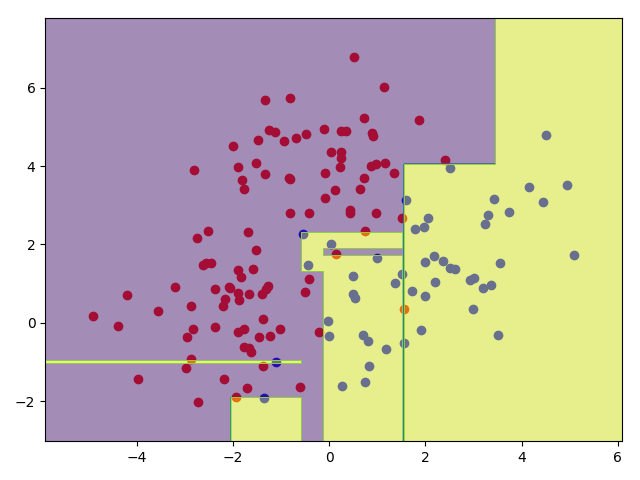
\includegraphics[width=.5\textwidth]{images/related_work/decision_tree_separator}
                    \caption{
                        \label{fig::decision_tree_separator} Visualization of a decision tree separator trained over generated data in a two dimensional feature space.
                        The separator is composed exclusively of horiontal and vertical lines.
                        We can also see how the decision tree overfits by adding narrow splits to accomodate lone points surrounded by others with an opposite class.
                    }
                \end{figure}

                The decision tree classier consists on successive conditions.
                It is easily modeled as a tree graph rooted at $r$.
                Each non leaf node $b$ in tree has as input an observation $\bm{x}$ which is fed to logical predicate $P_b$.
                Since we work with a first order logic\footnote{$P_b(\bm{x})$ can takle only two values.}, exactly two children are possible per node.
                These predicates are very specific: only on one dimension $i_b$ of the data is taken into account.
                The output is then computed by applying a threshold $t_b$ to $x_{i_b}$.
                This can be simplifief as $P_b(\bm{x}) = \mathbb{1}_{x_{i_b} \geq t_b} $.
                The chosen child is denoted $d_b(\bm{x}) \leftarrow \text{child}(b, \mathbb{1}_{x_{i_b} \geq t_b})$.
                Leafs do not apply any predicate to their input.
                Instead, based on their assigned class $c(l) \in \{1,2,\dots,C\}$ of the leaf $l$, they predict the label of the input.
                The each dimension $x_i \in \mathscr{X}_i$ is treated separately.
                Hence, decision trees can handle heterogenous feature vectors that are no longer restricted to be $\mathbb{R}^d$.
                The decision function of a decision tree classier can be written as:
                \begin{equation}
                    \label{eq::df_decision_tree}
                    \begin{aligned}
                        D_{\text{decision tree}}: \prod_{i=1}^{d}\mathscr{X}_i &\rightarrow \{1,2,\dots,C\}\\
                        \bm{x} &\mapsto c\left(d_{d_{\ddots_{d_r(\bm{x})}}(\bm{x})}\right)
                    \end{aligned}
                \end{equation}
                This representation is complicated and too abstract.
                In Figure~\ref{fig::decision_tree_graph}, is illustrated a typical and intuitive representation of decision tree classiers.
                In Figure~\ref{fig::decision_tree_separator}, we can clearly attribute the fact that the separator is an aggregation of vertical and horiontal segments to the fact that only one dimension is taken into acoount at a time.\\

                Up to now, we assumed the fact that the decision tree is already in place.
                First, it should be trained: \textit{i.e.} we have to determine its structure and all the thresholds.
                The goals is to have leaves with no prediction errors.
                As a consequence, all obsevations that end up in this leaf must be of the same class: the leaf is called pure.
                While a node is not pure, it will not be a leaf.
                In order to determine its spliting threshold, is chosen the one that has the most gain in ``purity''.
                Consequently, there is a need of a metric $I$ that can describe the heterogenuity of a node.
                These are usually based on a probabilistic interepretation as we compute the fraction of observations $p_c$ that go through a node of class $c \in \{1, 2, \dots, C\}$.
                Three examples are provided:
                \begin{itemize}
                    \item Gini index:
                    \begin{equation}
                        \label{eq::gini}
                        I_G\left(\left(p_c\right)_{c=1, 2, \dots, C}\right) = \sum_{c=1}^{C} p_c \cdot \sum_{\substack{l=1, 2, \dots, C\\l \neq c}} p_l;
                    \end{equation}
                    \item Entropy:
                    \begin{equation}
                        \label{eq::entropy}
                        I_H\left(\left(p_c\right)_{c=1, 2, \dots, C}\right) = - \sum_{c=1}^{C} p_c \cdot \log_2(p_c);
                    \end{equation}
                    \item Variance:
                    \begin{equation}
                        \label{eq::variance_index}
                        I_V\left(\left(x_p^i\right)_{i\in S}\right) = \frac{1}{2 \cdot \vert S \vert^2} \cdot \sum_{(i,j) \in S\times S} \left(x_p^i - x_p^j\right),
                    \end{equation}
                    where:
                    \begin{conditions}
                        p & is the chosen dimension to split over;\\
                        S & $\subset \{1, 2, \dots, n\}$ is a set of indices.
                    \end{conditions}
                \end{itemize}
                If we consider $S_b$ the set of indices of input going through a node $b$, we can compute the gain of a split at node $b$ as:
                \begin{equation}
                    \label{eq::split_gain}
                    G_b \triangleq I(S_b) - \sum_{c \in \{d_b(\bm{x}^i): i \in S_b\}} I(S_c)
                \end{equation}
                The optimal threshold is chosen so that it maximizes the gain $G_b$.\\
                Stoping only when total purity is achieved can yield complicated decision trees that overfit easily.
                This motivates the use for early stoping criteria:
                \begin{itemize}
                    \item a minimal number of observations going through each node.
                    \item a minimal purity ratio computed as the ratio of all instances going through the node having the dominant class.
                    \item a maximal depth of the tree.
                \end{itemize}
                To conclude, the class at each leaf is taken as the dominant class of instances entering it.

            \paragraph{Bagging decision trees}
                \begin{figure}
                    \centering
                    \includestandalone[mode=buildnew, height=.4\textheight]{figures/random_forest/bagging}
                    \caption{
                        \label{fig::bagging} Illustration of the principle of bagging.
                        For each decision function $\forall l=1,2,3\;D_l$, is represented the instances where the classier fails $F(D_l) \rightarrow \{(\bm{x}, y) \in \prod_{i=1}^{d}\mathscr{X}_i \times \{1,2,\dots,C\} : D_l(\bm{x}) \neq y\}$.
                        In the case of unweigthed bagging, the aggregated classier will fail when more than half the classiers fail.
                        In this case, the set $F(D_{\text{bagging}})$ is the union of intersections of two different $F(D_l)$: $F(D_{\text{bagging}}) = \bigcup_{l\neq p} F(D_l) \cap F(D_p)$.
                        In this case classiers are diverse and, as a consequence, the aggregated classier fails less frequently than a single one.
                    }
                \end{figure}

                \begin{figure}
                    \centering
                    \ffigbox[\FBwidth]{
                        \begin{subfloatrow}[2]
                            \ffigbox[\FBwidth]{
                                \includestandalone[mode=buildnew, width=.45\textwidth]{figures/random_forest/circles_dt}
                            }{
                                \caption{
                                    \label{fig::decision_tree_circles} Decision tree separator.
                                }
                            }
                            \ffigbox[\FBwidth]{
                                \includestandalone[mode=buildnew, width=.45\textwidth]{figures/random_forest/circles_rf}
                            }{
                                \caption{
                                    \label{fig::rf_circles} Random forest separator (in purple) with constituing decision trees.
                                }
                            }
                        \end{subfloatrow}
                    }{
                        \caption{
                            \label{fig::decision_tree_vs_rf} Difference betwwen a single decision tree and a random forest visualized in feature space for a generated toy data.
                            We see how a random forest aggregates multiple shallow decision trees in order to achieve a good generalization power instead of overfitting to the sampled data.
                        }
                    }
                \end{figure}

                While reducing the complexity of the decision tree can help avoid overfitting problems, one can risk an underfitting in the classification.
                In order to find a compromise, a bagging strategy can be adopted.
                The principle of bagging is to multiply different underperforming classiers and aggregate them together.
                These classiers should be taken as diverse as possible in order to cover the whole feature space.
                The aggregation is achieved through a majority vote and, if the classiers can provide probabilities, the vote can be weighted.
                This is illustrated in Figure~\ref{fig::bagging}.
                Mathematically the decision function of an unweighted aggregation of classifiers $\left(D_l\right)_{l=1,2,\dots,L}$ can be written as:
                \begin{equation}
                    \label{eq::decision_function_hard_bagging}
                    \begin{aligned}
                        D_{\text{hard bagging}, \left(D_l\right)_{l=1,2,\dots,L}}: \prod_{i=1}^{d}\mathscr{X}_i &\rightarrow \{1,2,\dots,C\}\\
                        \bm{x} &\mapsto \arg \max_{c=1,2,\dots,C}\lvert\{l\in\{1,2,\dots,L\}: D_l(\bm{x}) = c\}\rvert
                    \end{aligned},
                \end{equation}
                while the weighted aggregation using classifier output probabilities $\left(p_l\right)_{l=1,2,\dots,L}$ is expressed as:
                \begin{equation}
                    \label{eq::decision_function_weighted_bagging}
                    \begin{aligned}
                        D_{\text{weighted bagging}, \left((D_l, p_l)\right)_{l=1,2,\dots,L}}: \prod_{i=1}^{d}\mathscr{X}_i &\rightarrow \{1,2,\dots,C\}\\
                        \bm{x} &\mapsto \arg \max_{c=1,2,\dots,C} \sum_{l=1}^{L} p_l\left(D_l(\bm{x}) = c\right) 
                    \end{aligned}.
                \end{equation}
                Multiple decision trees are trained where each one hopefull specializes in a certain pattern.
                This possible by randomly selecting a subset of the features when learning spliting thresholds.
                We depict in Figure~\ref{fig::decision_tree_vs_rf} the different between a random forest and a single decision tree.
            \paragraph{Properties}
    \subsection{Computer vision}
        \label{subsec::state_of_the_art::mlpr::computer_vision}

        \subsubsection{Edge detection}
            Edges in images virtual curves that delimits objects.
            Edge detection has been well studied for a long time in image processing and computer vision fields.
            Actually, an edge is defined formally as a sharp change in the image signal.
            Once detected they can be used for many applications.
            One such use is building modeling.
            As seen previously, buildings can be modeled fairly as piecewise planar surfaces.
            As a consequence, one important building geometric feature are segments resulting from intersections of such surfaces.
            Hence the wide use of edge detection as a proxy for building \gls{acr::3d} modeling.
            The goal of this sub-subsection is not to provide a thorough survey of edge detection techniques, but rather, explain the basic ideas behind.\\
            
            A natural way to detect discontinuities in the signal is to compute gradients and look for high amplitudes.
            Indeed, one can apply Sobel filters\footnote{which correspond to a discretization of partial derivatives $\frac{\partial}{\partial x}$ and $\frac{\partial}{\partial y}$ respectively.}
            \begin{equation}
                \label{eq::sobel_filters}
                \begin{cases}
                    S_x \triangleq \begin{bmatrix}
                        -1 & 0 & 1\\
                        -2 & 0 & 2\\
                        -1 & 0 & 1
                    \end{bmatrix}\\
                    S_y \triangleq \begin{bmatrix}
                        -1 & -2 & 1\\
                        0 & 0 & 0\\
                        -1 & 2 & 1
                    \end{bmatrix}\\
                \end{cases}
            \end{equation}
            to an image $I$.
            Afterwards are retrieved the gradient amplitudes per pixel:
            \begin{equation}
                \label{eq::sobel_amplitude}
                G = \sqrt{\left(S_x\star I\right)^2 + \left(S_y\star I\right)^2},
            \end{equation}
            where the operations are applied term-wise.
            However, edges are not the only feature relating to high gradient amplitudes.
            Noise results also in small amplitude discontinuities in the image.
            In order to filter out noise, one can apply low frequency filters that smooths the image.
            For instance, one can apply Gaussian filters.
            These should be tuned in so that they eradicate most of the noise without smudging edges.
            The same basic idea is used again for line segment detction for instance~\parencite{von2008lsd}.
            Other approaches are possible but are discussed herein, such as wavelet based approaches~\parencite{mallat1992singularity}.

        \subsubsection{\acrlong*{acr::scatnet}}
            \glspl{acr::scatnet} are convolutional networks built using wavelet filters for image feature extraction.
            Contrarily to \glspl{acr::cnn}, \glspl{acr::scatnet} seek an image representation $\Phi$ without relying on supervized learning, but rather using mathematical properties of the signal.
            A scene that is captured from different point of views, while yielding different images, should have the same representation.
            Just as with interset point detection~\parencite{harris1988combined,lowe1999object}, the representation of an image should be invariant to scale, translation and rotation~\parencite{mallat2012group,sifre2013rotation,bruna2013invariant}.
            Let $x$ be an image and $G$ a group such as a translatin group.
            The action of $g\in G$ on $x: u \mapsto x(u)$ is written as:
            \begin{equation}
                \label{eq::action_group}
                L_g(x): u \mapsto x\left(g^{-1}(u)\right).
            \end{equation}
            $\Phi$ is said to be invariant to $g$ if and only if:
            \begin{equation}
                \label{eq::invariance}
                \Phi\circ L_g\left(x\right) = \Phi(x),
            \end{equation}
            and covariant if and only if:
            \begin{equation}
                \label{eq::covariance}
                \Phi\circ L_g\left(x\right) = L_g\circ\Phi(x).
            \end{equation}
            Images of similar objects should have a representations that are also similar.
            Using Euclidean distances as a similarity measure, this property implies $\Phi$ to be contractive~\parencite{bruna2013invariant}.
            Given two images $x$ and $y$, we write:
            \begin{equation}
                \label{eq::contractive}
                \Vert \Phi(x) - \Phi(y) \Vert \leq \Vert x-y \Vert.
            \end{equation}
            Since images are subject to distortions and not all objects are rigid, the mapping $\Phi$ should be stable under small deformations~\parencite{bruna2013invariant,sifre2013rotation,mallat2012group}.
            Given a small deformation modelled as a diffeomorphism\footnote{A differentiable bijection which inverse is differentiable also.} $\tau$ such that $\Vert\nabla \tau\Vert_\infty < 1$, there exists a constant $C>0$ such that for any image $x$:
            \begin{equation}
                \label{eq::stable_deformation}
                \Vert \Phi(x) - \Phi\circ L_\tau(x) \Vert \leq C \cdot \Vert x\Vert \cdot \Vert\nabla \tau\Vert_\infty.
            \end{equation}
            where:
            \begin{conditions}
                L_\tau(x) & $u \mapsto x(u - \tau(u))$ is the action of the deformation $x$ on a signal $x$.
            \end{conditions}

            \glspl{acr::cnn} learn a representation that verifies these previous conditions stated in Equations~\ref{eq::invariance},~\ref{eq::contractive} and~\ref{eq::stable_deformation}.
            In fact, \glspl{acr::cnn} are indeed are made invariant to translations and local deformations up to a scale mainly due to the pooling layers.
            Since the weights are learned based on a classification objetive, images with similar content are supposed to be mapped to the same region.
            A \gls{acr::scatnet} can be seen as a reverse engineered \gls{acr::cnn}.
            The idea is to apply linear convolutional operators followed by a non-linearity and some pooling operators.
            In a \gls{acr::scatnet} the learned filters are replaced by a specific wavelet decomposition, the non-linearity is acheived using the modulus operator and pooling is obtained through a low pass filter.
            The low-pass filter is critical for the invariance condition, while the high frequencies are extracted using the wavelet convolutions.
            The non-linearity, just in \glspl{acr::cnn}, is necessary in order to obtain interesting non-linear representations.\\

            Based on a band-pass filter $\psi$ one can generate a two-dimentional wavelet filter bank using rotations $r$ and dilatations of scale $j$:
            \begin{equation}
                \label{eq::filter_bank}
                \psi_{j,r} = 2^{-2\cdot j}\cdot\psi\left(2^{-j}\cdot r^{-1}(u)\right).
            \end{equation}
            When the Fourier transform of $\psi$ is centred at a frequency $\omega$, the wavelet $\psi_{j,r}$ is centered around $\left(2^{-j}\cdot r(\omega)\right)$ with bandwidth propotional to $2^{-j}$.
            Based on these filters is computed the wavelet transform of a signal $x$: $\{x\star\psi_{j,r}\}_{j,r}$.
            Morlet wavelets and a Gaussian low-pass filter are usual choices~\parencite{bruna2013invariant,sifre2013rotation}.
            The basic bloc of a \gls{acr::scatnet} is the wavelet-modulus operator:
            \begin{equation}
                \label{eq::basic_operator}
                U_{j,r}(x) = \vert x\star\psi_{j,r} \vert.
            \end{equation}
            This can be reapplyed successively like with \glspl{acr::cnn} at different scales and rotations:
            \begin{equation}
                \label{eq::basic_operator}
                U[p](x) = U_{j_m,r_m}\circ U_{j_{m-1},r_{m-1}} \circ \dots U_{j_1,r_1} (x),
            \end{equation}
            where:
            \begin{conditions}
                p & is called a path and is the sequence of parameters $\left((j_i, r_i)\right)_{i=1,2,\dots,m}$.
            \end{conditions}
            A scattering transform at a path $p$ consists in a pooling of the the successive wavelet-modulus operators, using a scaled low-pass filter $\phi_J: u\mapsto 2^{-2\cdot J}\cdot\phi\left(2^{-\cdot J}\cdot u\right)$:
            \begin{equation}
                \label{eq::scattering_transform}
                S_J[p](x) \triangleq U[p](x) \star \phi_J
            \end{equation}

            If these filters can cover the whole frequency space then the scattering transform is invertible.
            Moreover, the scattering tranform can be proved to verify all the required conditions~\parencite{mallat2012group}.
            The convolution depends on the choice of the group $G$.
            For images, scaling can be diassociated from rotations and translations.
            This is not true between rotations and translations~\parencite{sifre2013rotation,oyallon2015deep}.
            Convolutions are computed on $G$:
            \begin{equation}
                \label{eq::group_convolution}
                x\star y(g) = \int_{h\in G} x(h)\cdot y(h^{-1}*g)
            \end{equation}
            A logarithm is applied then to the scattering coefficients as well as a global scale space averaging in order to obtain a global image descriptor.

            \begin{figure}
                \centering
                \includestandalone[mode=buildnew, width=\textwidth]{figures/scattering_network}
                \caption{
                    \label{fig::scatnet} Illustration of a \gls{acr::scatnet}.
                    At each level are computed are computed convolutions with a filter bank followed by a modulus operator.
                    The scattering coefficients are obtained then by a low-pass filter (in blue).
                    In practice, not all scattering coefficients are computed.
                }
            \end{figure}

            In Figure~\ref{fig::scatnet} is represented the \acrlong{acr::scatnet}.
            The number of scattering coefficients is exponential in the network depth.
            Usually, not all coefficients are computed.
            Instead they are computed following a non decreasing frequency path.
            Moreover, most of the energy of the signal is contained in the first two layers.
            This is why, in practice, the computation is stopped at that level.

        \subsubsection{Convolutional neural networks}
    \subsection{Graph classification}
        \label{subsec::state_of_the_art::mlpr::graph_classification}

        \subsubsection{Graph kernels}
        \subsubsection{Graph neural networks}
